\chapter{Progettazione}
La fase di progettazione prevede principalmente la scelta dell'architettura da usare, su cui costruire il sistema. Dopo averla definita in modo chiaro si 

\section{Architettura}
La progettazione dell'architettura si divide in:
\begin{itemize}
	\item Stile Architetturale
	\item Pattern Architetturale
\end{itemize}

\subsection{Stile Archietturale}
Lo stile scelto per la realizzazione del sistema è una composizione tra \textbf{Blackboard}, uno stile di tipo \textit{shared memory} e \textbf{Publish-Subscribe}, stile di tipo \textit{implicit invocation}.

\subsubsection{Blackboard}
L'idea è quella di avere una "lavagna" in cui una tipologia di dipendente scrive e un'altra tipologia, invece, legge.
Ad esempio un cameriere (dipendente di sala) scrive un'ordinazione sulla lavagna e i cuochi, pizzaioli (realizzatori di ordinazioni) possono leggere per vedere cosa il cameriere ha scritto e iniziare a preparare le pietanze.
\\Il problema di questo stile puro è che i dipendenti hanno bisogno di sapere in real-time quando c'è una modifica \textit{asincrona} alla lavagna. Una possibile soluzione è quella di implementare un'attesa attiva per controllare constantemente lo stato della lavagna, particolarmente inefficiente. 
\\Una seconda possibilità è quella di modificare lo stile architetturale aggiungendo una parte di stile \textit{event-based}.

\subsubsection{Publish-Subscribe}
L'idea è quella di notificare in tempo reale tutti i dispositivi che hanno bisogno di leggere dalla lavagna, disaccoppiandoli a loro volta. 

\section{Database}
Il database deve contenere le informazioni di base che devono essere utilizzate, a partire dai dipendenti che vengono registrati nel sistema e finire con le ordinazioni che vengono effettuate durante l'utilizzo del sistema.
\begin{figure}[H]
	\centering
	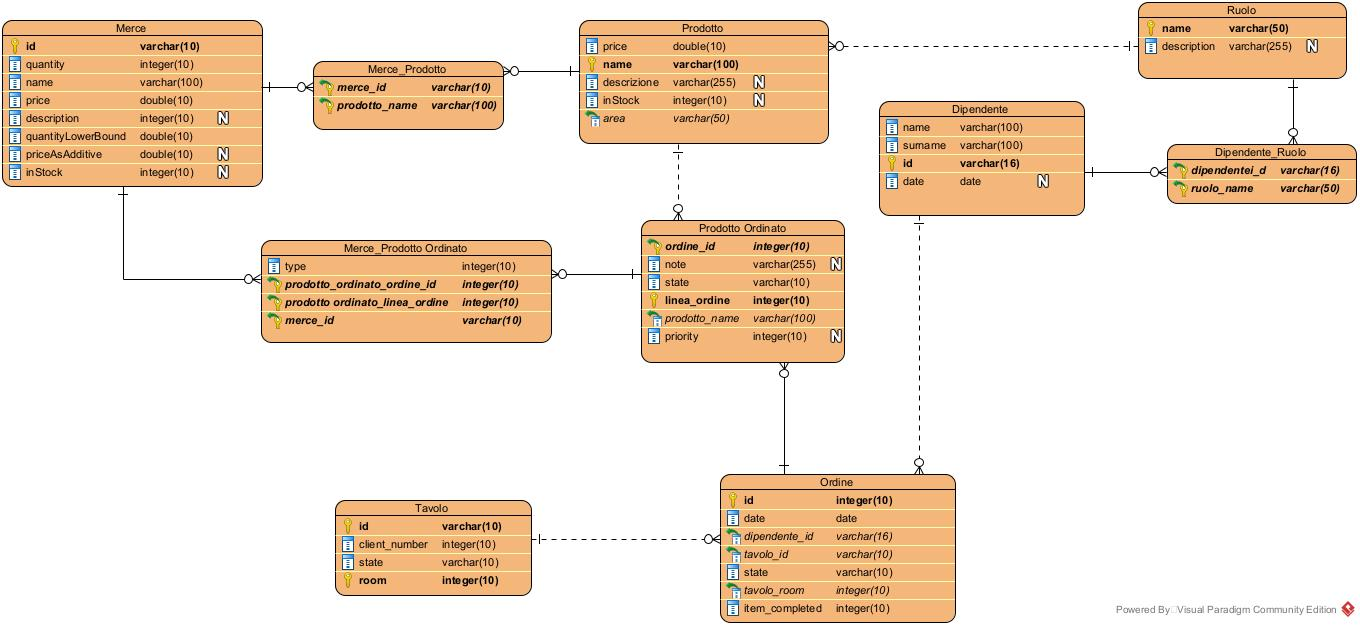
\includegraphics[width=1\textwidth]{Immagini/database.jpg}
\end{figure}
Le caratteristiche principali del database sono le seguenti:
\begin{enumerate}
	\item Le merci hanno, oltre alle informazioni di base quali prezzo, codice identificativo, nome, etc, hanno un attributo \textit{priceAsAdditive}. Tale attributo, se non nullo, indica il prezzo da aggiungere se quella merce è usata come merce aggiuntiva di un prodotto.
	\item Il \textit{Prodotto Ordinato} è un'associazione ternaria tra \textit{Ordine}, \textit{Prodotto} e \textit{Merce}.
	 \item Ogni prodotto ha un attributo collegato all'entità \textit{Ruoli}. Esso serve per indicare a che attività appartiene quel prodotto.
\end{enumerate}
Il precedente database si riferisce solo ai casi d'uso che si sono scelti di implementare. Non contiene, ad esempio, la gestione delle vendite e lo storico del locale.

\section{Component Diagram}
\begin{figure}[H]
	\centering
	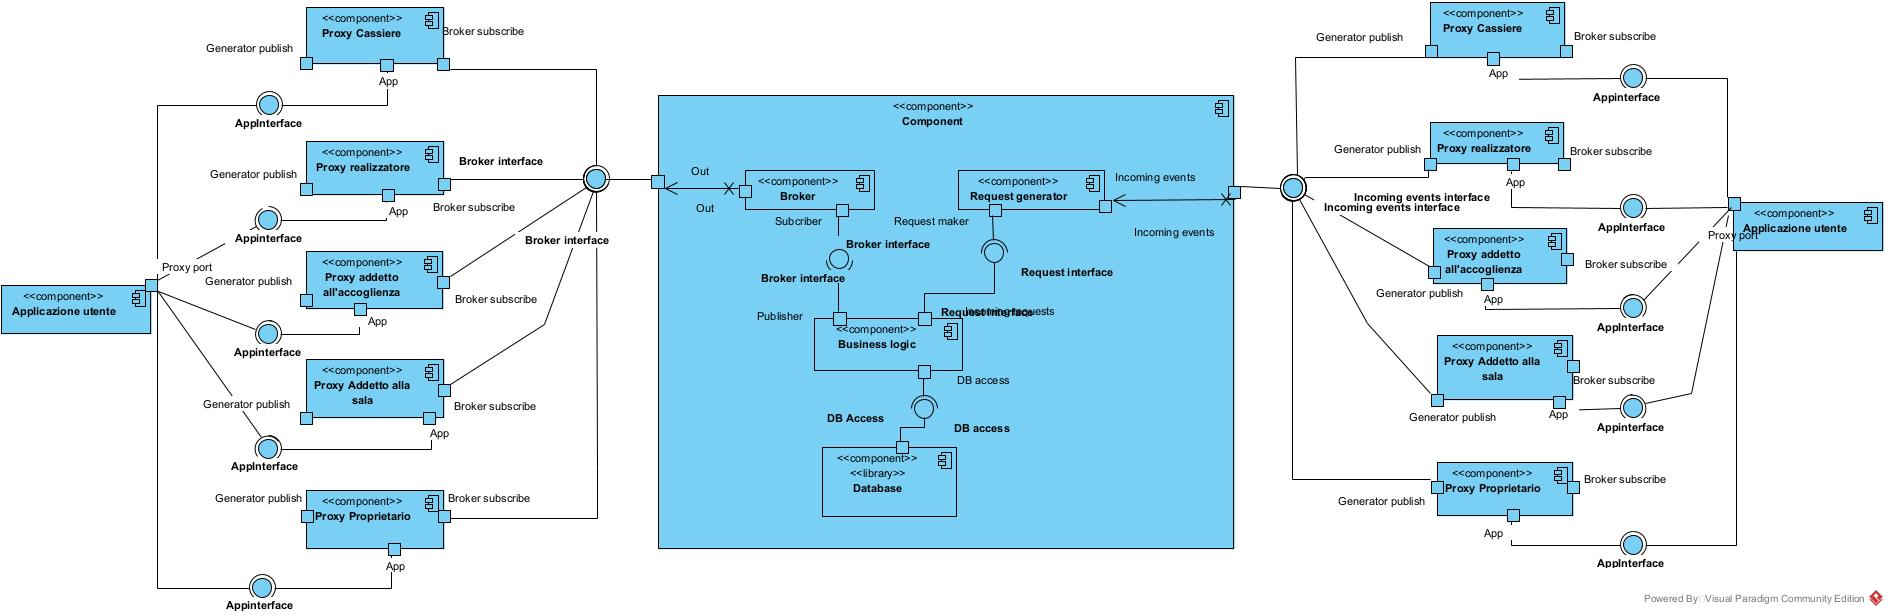
\includegraphics[width=1\textwidth]{Immagini/dynamic components.jpg}
\end{figure}
\section{Deployment Diagram}
\section{Class Diagram}
\section{Sequence Diagram}